\section{Đề ôn thi giữa kỳ 2 toán 10}
\subsection{Câu trắc nghiệm đúng sai}
Học sinh trả lời từ câu 1 đến câu 4.
Trong mỗi ý \circlenum{A}, \circlenum{B}, \circlenum{C} và \circlenum{D} ở mỗi câu, học sinh chọn đúng hoặc sai.
\setcounter{ex}{0}
\LGexTF
\Opensolutionfile{ansbook}[ansbook/DapanDS]
\Opensolutionfile{ans}[Ans/DapanT]

%%%=============EX_1=============%%%

\begin{ex}%[0D7N2-2]%[1-Dự án đề kiểm tra Khối 10 - GHKII - NH23-24- Đợt 2 - VU Ngoc Hao]%[Đề số 3 - CTST]
 Cho hàm số bậc hai $y=f(x)$ có đồ thị như hình vẽ sau:
 \begin{center}
 	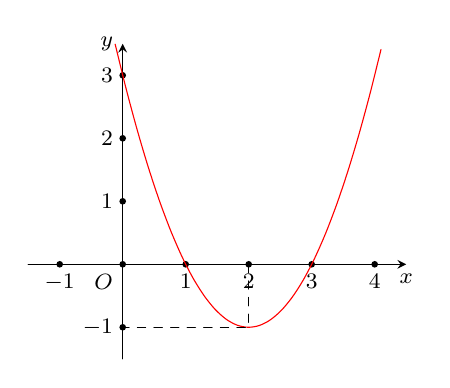
\begin{tikzpicture}[scale=0.8, font=\footnotesize, line join=round, line cap=round, >=stealth,
 		declare function={
 			f(\x)=(\x)^2-4*(\x)+3;
 		}
 		]
 		%\draw[gray!10] (-1,-1) grid (5,5);
 		\draw[->] (-1.5,0)--(4.5,0) node[below]{$x$};
 		\draw[->] (0,-1.5)--(0,3.5) node[left]{$y$};
 		\fill (0,0) node[below left]{$O$} circle(1.5pt);
 		\foreach \p in {-1,1,2,3,4}
 		\fill (\p,0) circle (1.5pt) node[below]{$\p$};
 		\foreach \r in {-1,1,2,3}
 		\fill (0,\r) circle (1.5pt) node[left]{$\r$};
 		\draw[smooth,red] plot[domain=-0.12:4.1] ({\x},{f(\x)});
 		\draw[dashed] (2,0)--(2,-1)--(0,-1);
 	\end{tikzpicture}
 \end{center}
 Nhận định nào sau đây là đúng?
 \choice
 {Bất phương trính $f(x)>0$ nghiệm đúng với mọi $x>1$}
 {Phương trình $f(x)=0$ có hai nghiệm là $x=0$ và $x=1$}
 {\True Bất phương trình $f(x)<0$ có tập nghiệm là $S=(1;3)$}
 {Bất phương trình $f(x)>0$ có tập nghiệm là $S=(1;3)$}
 \loigiai{
 Bất phương trình $f(x)<0 \Leftrightarrow 1<x<3.$\\
 Vậy bất phương trình $f(x)<0$ có tập nghiệm là $S=(1;3)$.
 }
 \end{ex}
\begin{ex}%[0D7N1-2]%[1-Dự án đề kiểm tra Khối 10 - GHKII - NH23-24- Đợt 2 - VU Ngoc Hao]%[Đề số 3 - CTST]
Tam thức bậc hai nào sau đây luôn nhận giá trị dương với mọi $x \in \mathbb{R}$?
 \choice
  {$x^2-3 x+2$}
  {$x^2-4 x+3$}
  {$-x^2+x-1$}
  {\True $x^2-3 x+3$}
   \loigiai{
  Xét $f(x)=x^2-3 x+3$, ta có $a=1>0$, $\Delta = (-3)^2-4\cdot 1\cdot 3 = -3 <0$ nên $f(x)=x^2-3 x+3<0$ với mọi $x \in \mathbb{R}$.
  }
\end{ex}  
\begin{ex} %[0D7N2-1]%[1-Dự án đề kiểm tra Khối 10 - GHKII - NH23-24- Đợt 2 - VU Ngoc Hao]%[Đề số 3 - CTST]
	Tập nghiệm của bất phương trình $x^2-5x+6>0$ là
	 \choice
  {\True $S=(-\infty ; 2) \cup(3 ;+\infty)$}
  {$S=(-\infty ; 3)$}
  {$S=(2 ; 3)$}
  {$S=(2 ;+\infty)$}
  \loigiai{
  Bất phương trình $x^2-5x+6>0$.\\
  Bảng xét dấu \begin{center}
  	
\begin{tikzpicture}
  	\tkzTabInit[nocadre=false,lgt=2,espcl=2,deltacl=0.6]
  	{$x$ /0.6,$f(x)$ /0.6}
  	{$-\infty$,$2$,$3$,$+\infty$}
  	\tkzTabLine{,+,$0$,-,$0$,+,}
  \end{tikzpicture}
  \end{center}
   Vậy bất phương trình có tập nghiệm là $S=(-\infty ; 2) \cup(3 ;+\infty)$.
  }
\end{ex}  
\begin{ex}%[0D7N1-2]%[1-Dự án đề kiểm tra Khối 10 - GHKII - NH23-24- Đợt 2 - VU Ngoc Hao]%[Đề số 3 - CTST]
Tam thức bậc hai $f(x)=-x^2+5 x-6$ nhận giá trị âm với $x$ thuộc khoảng nào dưới đây?
 \choice
  {$x \in(-\infty ; 3)$}
  {\True $x \in (3 ;+\infty)$}
  {$x \in(2 ;+\infty)$}
  {$x \in(2 ; 3)$}
  \loigiai{
 Ta có $f(x)=-x^2+5 x-6<0 \Leftrightarrow x^2-5 x+6>0$.\\
 Bảng xét dấu \begin{center}
 	
\begin{tikzpicture}
 		\tkzTabInit[nocadre=false,lgt=2,espcl=2,deltacl=0.6]
 		{$x$ /0.6,$f(x)$ /0.6}
 		{$-\infty$,$2$,$3$,$+\infty$}
 		\tkzTabLine{,+,$0$,-,$0$,+,}
 	\end{tikzpicture}
 \end{center}
 Vậy tam thức bậc hai $f(x)=-x^2+5 x-6$ nhận giá trị âm với $x \in (3 ;+\infty)$.
 } 
\end{ex}  
\begin{ex}%[0D7H3-2]%[1-Dự án đề kiểm tra Khối 10 - GHKII - NH23-24- Đợt 2 - VU Ngoc Hao]%[Đề số 3 - CTST]
	Tập nghiệm của phương trình $\sqrt{5 x^2-6 x-4}=2(x-1)$ là
  \choice
  {$S=\{-4\}$}
  {$S=\{-4 ; 2\}$}
  {$S=\{1\}$}
  {\True $S=\{2\}$}
  \loigiai{
  Điều kiện $x\ge1$.\\
  Bình phương 2 vế ta được $5 x^2-6 x-4=4x^2-8x+4\Leftrightarrow x^2+2x-8=0 \Leftrightarrow \hoac{&x=-4\\&x=2.}$\\
  Kiểm tra điều kiện ta nhận nghiệm $x=2$.
  
  }
\end{ex}  
\begin{ex}%[0D7H3-2]%[1-Dự án đề kiểm tra Khối 10 - GHKII - NH23-24- Đợt 2 - VU Ngoc Hao]%[Đề số 3 - CTST]
	Số nghiệm của phương trình $\sqrt{4 x+7}=2 x-1$ là
	 \choice
   	{\True $1$} 
  	{$2$} 
  	{$3$} 
   	{$0$} 
   \loigiai{
   Điều kiện $x\ge\dfrac{1}{2}$.\\
   Bình phương 2 vế ta được $4x+7=4x^2-4x+1\Leftrightarrow 2x^2-4x-3=0 \Leftrightarrow \hoac{&x=\dfrac{2-2\sqrt{6}}{2}\\&x=\dfrac{2+2\sqrt{6}}{2}.}$\\
   Kiểm tra điều kiện ta nhận nghiệm $x=\dfrac{2+2\sqrt{6}}{2}$.		
   	}
\end{ex}

%%%============EX_1==============%%%
\begin{ex}%[0H1Y2-1]%[Dự án đề kiểm tra Toán khối 10 GHKII NH23-24-Dot 1-Nguyễn Duy]%[Deso 3 - CTST]
	Trong mặt phẳng tọa độ $Oxy$, cho ba điểm $A(-1{;} 2)$, $B(2{;}-2)$, $C(3{;} 1)$. Toạ độ của vectơ $\overrightarrow{AB}+\overrightarrow{BC}$ là:
	\choice
	{$(-4{;}-1)$}
	{\True$(4{;}-1)$}
	{$(-4{;} 1)$}
	{$(4{;} 1)$}
	\loigiai{%
		Áp dụng quy tắc ba điểm, ta có:$\overrightarrow{AB} + \overrightarrow{BC} =\overrightarrow{AC}=(x_{\mathrm{C}}-x_\mathrm{ A}{;}y_\mathrm{C}-y_\mathrm{A})=(4{;}-1)$ 
	}
\end{ex}
%%%============EX_8==============%%%
\begin{ex}%[0H1B2-1]%[Dự án đề kiểm tra Toán khối 10 GHKII NH23-24-Dot 1-Nguyễn Duy]%[Deso 3 - CTST]
	Trong mặt phẳng tọa độ $Oxy$, cho ba điểm $A(-1{;} 2)$, $B(0{;}-2)$, $C(3{;} 3)$. Toạ độ của vectơ $2\overrightarrow{AB}-4\overrightarrow{BC}$ là:
	\choice
	{$(14{;}12)$}
	{\True$(-10{;}-28)$}
	{$(-14{;}-12)$}
	{$(10{;}28)$}
	\loigiai{%
		\par Ta có: $\overrightarrow{AB}=(x_{B}-x_{A};y_{B}-y_{A})=(1;-4)\Rightarrow 2\overrightarrow{AB}=(2;-8)$.
		
		$\overrightarrow{BC}=(x_{C}-x_{B};y_{C}-y_{B})=(3;5)\Rightarrow -4\overrightarrow{BC}=(-12;-20)$.
		
		Vậy $2\overrightarrow{AB}-4\overrightarrow{BC}=(2-12;-8-20)=(-10;-28)$
	}%
\end{ex}
%%%============EX_9==============%%%
\begin{ex}%[0H3B1-2]%[Dự án đề kiểm tra Toán khối 10 GHKII NH23-24-Dot 1-Nguyễn Duy]%[Deso 3 - CTST]
	Phương trình tham số của đường thẳng đi qua $A(-2{;}1)$, nhận $\overrightarrow{u}=(3{;}-1)$ làm vectơ chỉ phương là
	\choice
	{\True$\heva{&x=-2+3t \\ & y=1-t}$}
	{$\heva{&x=3-2t \\ & y=-1+t}$}
	{$3x-y+7=0$}
	{$-2x+y+7=0$}
	\loigiai{%
		\begin{itemize}
			\item \textbf{Kiến thức cần nhớ:} Phương trình tham số của đường thẳng $(d)$ đi qua $M(x_0;y_0)$ và nhận $\overrightarrow{u}=(a;b)$ làm véc tơ chỉ phương là $\heva{&x=x_0+at \\ & y=y_0+bt}$.\\
			\item \textbf{Áp dụng:} Phương trình tham số của đường thẳng đi qua $A(-2{;}1)$, nhận $\overrightarrow{u}=(3{;}-1)$ làm vectơ chỉ phương là $\heva{&x=-2+3t \\ & y=1-t}$
		\end{itemize}
	}%
\end{ex}
%%%============EX_10==============%%%
\begin{ex}%[0H3T1-7]%[Dự án đề kiểm tra Toán khối 10 GHKII NH23-24-Dot 1-Nguyễn Duy]%[Deso 3 - CTST]
	\immini{Fahrenheit là một thang đo nhiệt độ nhiệt động lực học, với điểm đóng băng của nước là $32$ độ F $\left(^{\circ} \mathrm{F}\right)$ và điểm sôi là $212^{\circ} \mathrm{F}$ (ở áp suất khí quyển tiêu chuẩn). Việc quy đổi nhiệt độ giữa đơn vị độ C và đơn vị độ F được xác định bởi hai điểm trên mặt phẳng tọa độ: Điểm đóng băng của nước là $(0{;}32)$ và Điểm sôi của (Kết quả làm tròn đến chữ số hàng phần trăm)
		\choice
		{$23{,}56^{\circ}\mathrm{C}$}
		{$122{,}4^{\circ}\mathrm{C}$}
		{$37{,}78^{\circ}\mathrm{C}$}
		{$212^{\circ}\mathrm{C}$}}{
		
\begin{tikzpicture}[declare function={k=0.55;},font=\scriptsize,scale=k]
			\tikzset{pics/.cd,
				tC/.style={code={
						\begin{scope}[scale=k]
							\foreach \i in {-4,-3,...,5}{
								\pgfmathtruncatemacro{\it}{\i*10}
								\draw[thick,cyan!85!black] (0,\i)--++(10pt,0)node[right]{\it} ;
							}
							\foreach \i in {-3.5,-2.5,...,4.5}{
								\pgfmathtruncatemacro{\it}{\i*10}
								\draw[thick,cyan!85!black] (0,\i)--++(5pt,0)node[right]{} ;
							}
							\foreach \i in {-3.9,-3.8,...,4.8,4.9}{
								\pgfmathtruncatemacro{\it}{\i*10}
								\draw[thin,cyan!85!black] (0,\i)--++(3pt,0)node[right]{} ;
							}
						\end{scope}
				}},
				tF/.style={code={
						\begin{scope}[scale=k]
							\foreach \i in {-4.0, -2.8889, -1.7778, -0.6667, 0.4444, 1.5556, 2.6667, 3.7778, 4.8889}{
								% Tính toán vị trí dựa trên giá trị Fahrenheit
								\pgfmathsetmacro{\pos}{int(round((\i*18)+32))}
								\draw[thick,cyan!85!black] (0,\i)--++(-10pt,0)node[left]{\pos} ;
							}
							\foreach \i in {-3.4444, -2.8889, -2.3333, -1.7778, -1.2222, -0.6667, -0.1111, 0.4444, 1.0, 1.5556, 2.1111, 2.6667, 3.2222, 3.7778, 4.3333}{
								\pgfmathsetmacro{\pos}{int(round((\i*18)+32))}
								\draw[thick,cyan!85!black] (0,\i)--++(-5pt,0)node[left]{} ;
							}
							\foreach \i in {-3.8889, -3.7778, -3.6667, -3.5556, -3.4444, -3.3333, -3.2222, -3.1111, -3.0, -2.8889, -2.7778, -2.6667, -2.5556, -2.4444, -2.3333, -2.2222, -2.1111, -2.0, -1.8889, -1.7778, -1.6667, -1.5556, -1.4444, -1.3333, -1.2222, -1.1111, -1.0, -0.8889, -0.7778, -0.6667, -0.5556, -0.4444, -0.3333, -0.2222, -0.1111, 0.0, 0.1111, 0.2222, 0.3333, 0.4444, 0.5556, 0.6667, 0.7778, 0.8889, 1.0, 1.1111, 1.2222, 1.3333, 1.4444, 1.5556, 1.6667, 1.7778, 1.8889, 2.0, 2.1111, 2.2222, 2.3333, 2.4444, 2.5556, 2.6667, 2.7778, 2.8889, 3.0, 3.1111, 3.2222, 3.3333, 3.4444, 3.5556, 3.6667, 3.7778, 3.8889, 4.0, 4.1111, 4.2222, 4.3333, 4.4444, 4.5556, 4.6667, 4.7778,5}{
								\pgfmathsetmacro{\pos}{int(round((\i*18)+32))}
								\draw[thin,cyan!85!black] (0,\i)--++(-3pt,0)node[left]{} ;
							}
						\end{scope}
						
				}}
			}
			%%%===============================================================%%%
			\path[rounded corners=12pt,fill=white!85!black](-2.7,-6.5)--++(0,13.25)-|(1.7,-6.5)--cycle;
			\path(0,0) pic[local bounding box=Cencius]  {tC};
			\path (Cencius.north) node[above,cyan!85!black] {$^{0}\textbf{\textsf{C}}$};
			\path(-1,0) pic[local bounding box=Fahrenheit]  {tF};
			\path (Fahrenheit.north) node[above,cyan!85!black,yshift =2pt] {$^{0}\textbf{\textsf{F}}$};
			
			\path (-0.5,-5)--+(75:0.8) coordinate (A)
			(-.5,-5)--+(-255:0.8) coordinate (B)
			(A)--+(0,10)coordinate(D)
			(A)--+(0,4.2)coordinate(E)
			(B)--+(0,4.2)coordinate(F)
			;
			\path [fill=red!55!pink] (A) arc (75:-255:0.8)--(F)--(E)--cycle;
			\path [draw=white!95!black,thick] (A) arc (75:-255:0.8)--++(0,10) coordinate(C)..controls +(90:10pt) and +(90:10pt) .. (D)--(A);
	\end{tikzpicture}}
	\loigiai{}
\end{ex}
%%%============EX_11==============%%%
\begin{ex}%[0H3B2-3]%[Dự án đề kiểm tra Toán khối 10 GHKII NH23-24-Dot 1-Nguyễn Duy]%[Deso 3 - CTST]
	Cho đường tròn $(C)$: $x^2+y^2+6x-4y-12=0$. Tiếp tuyến của đường tròn $(C)$ tại điểm $M(1;5)$ có phương trình là
	\choice
	{$4x-3y-19=0$}
	{\True$-4x-3y+19=0$}
	{$4x+3y+19=0$}
	{$-4x-3y-19=0$}
	\loigiai{
		\begin{itemize}
			\item \textbf{Kiến thức cần nhớ:} Phương trình đường tròn dạng $x^2+y^2-2ax-2ay+c=0$ có tâm $I(a;b)$ và bán kính $R=\sqrt{a^2+b^2-c}$.\\
			Phương trình tiếp tuyến của đường tròn tâm $I(a;b)$ tại $M(x_0;y_0)$ nằm trên đường tròn có phhương trình là $(a-x_0)(x-x_0) +(b-y_0)(y-y_0)=0$.
			\item \textbf{Áp dụng:} Phương trình đường tròn $x^2+y^2+6x-4y-12=0$ với $a=\frac{6}{-2}=-3$; $b=\frac{-4}{-2}=2$; $c=-12$ 
			
			$\Rightarrow$ tâm $I(-3;2)$ và bán kính $R=\sqrt{(-3)^2+2^2-(-12)}=5$. 
			
			Vì $1^2+5^2+6\cdot1-4\cdot5-12=5$ nên $M(1;5)$ nằm trên đường tròn.
			
			Vậy phương trình tiếp tuyến của nước $(\mathscr{C})$ tại $M$ là
			
		\end{itemize}
		\begin{eqnarray*}
			&&(-3-1)(x-1)+(2-5)(y-5)=0\\
			&\Leftrightarrow&-4(x-1)-3(y-5)=0\\
			&\Leftrightarrow&-4x-3y+19=0
		\end{eqnarray*}
	}
\end{ex}
%%%============EX_12==============%%%
\begin{ex}%[0H3K2-4]%[Dự án đề kiểm tra Toán khối 10 GHKII NH23-24-Dot 1-Nguyễn Duy]%[Deso 3 - CTST]
	Cho đường tròn $(C)$: $x^2+y^2-4x+6y-5=0$ và đường thẳng $\Delta$: $x+y+m=0$. Giá trị của $m$ để đường thẳng $\Delta$ tiếp xúc với đường tròn $(C)$ là
	\choice
	{\True$m=-5$ hoặc $m=7$}
	{$m=-8$ hoặc $m=13$}
	{$m=-15$ hoặc $m=21$}
	{$m=15$ hoặc $m=-8$}
	\loigiai{%
		
		Đường tròn $(\mathscr{C})$: $x^2+y^2-4x+6y-5=0$ có tâm $I(2;-3)$ và bán kính $R=\sqrt{2^2+(-3)^2+5}=3\sqrt{2}$.
		
		Đường thẳng $\Delta$ tiếp xúc với $(\mathscr{C})$ 
		\begin{eqnarray*}
			&\Leftrightarrow \ & d(I,\Delta) = R \\
			&\Leftrightarrow \ & \dfrac{|2+(-3+m)|}{\sqrt{1^2+1^2}}=3\sqrt{2}\\
			&\Leftrightarrow \ & |m-1|=6\\
			&\Leftrightarrow \ & m-1=6\ \text{hoặc} \ m-1=-6\\
			&\Leftrightarrow \ & m=7\ \text{hoặc} \ m=-5
		\end{eqnarray*}
	}
\end{ex}




\subsection{Câu trắc nghiệm đúng sai}
Học sinh trả lời từ câu 1 đến câu 4.
Trong mỗi ý \circlenum{A}, \circlenum{B}, \circlenum{C} và \circlenum{D} ở mỗi câu, học sinh chọn đúng hoặc sai.
\setcounter{ex}{0}
\LGexTF
\Opensolutionfile{ansbook}[ansbook/DapanDS]
\Opensolutionfile{ans}[Ans/DapanT]


\begin{ex}%[0D7H1-2]%[Dự án đề kiểm tra Toán khối 10 GHKII NH23-24-Dot 1- Thanh Hằng]%[Deso3- CTST]
	Xét tính đúng, sai của các khẳng định sau
	\choiceTF
	{\True $f(x)=x^2-x-2$ có $f(x)<0$ với mọi $x \in(-1 ; 2)$}
	{$f(x)=-x^2+2 x-5$ có $f(x)>0$ với mọi $x \in \mathbb{R}$}
	{\True $f(x)=-4 x^2+16 x-16$ có bảng xét dấu
		\begin{center}
			
\begin{tikzpicture}
				\tkzTabInit[nocadre=false,lgt=2,espcl=2,deltacl=0.6]
				{$x$ /0.6,$f(x)$ /0.6}
				{$-\infty$,$2$,$+\infty$}
				\tkzTabLine{,-,$0$,-,}
			\end{tikzpicture}
	\end{center}}
	{$f(x)=-4 x^2+3 x-5$ có bảng xét dấu
		\begin{center}
			
\begin{tikzpicture}
				\tkzTabInit[nocadre=false,lgt=2,espcl=2,deltacl=0.6]
				{$x$ /0.6,$f(x)$ /0.6}
				{$-\infty$,$-1$,$2$,$+\infty$}
				\tkzTabLine{,+,$0$,-,$0$,+,}
			\end{tikzpicture}
	\end{center}} 
	\loigiai{
		\begin{itemize}
			\item Bảng xét dấu của $f(x)=x^2-x-2$ là
			\begin{center}
				
\begin{tikzpicture}
					\tkzTabInit[nocadre=false,lgt=2,espcl=2,deltacl=0.6]
					{$x$ /0.6,$f(x)$ /0.6}
					{$-\infty$,$-1$,$2$,$+\infty$}
					\tkzTabLine{,+,$0$,-,$0$,+,}
				\end{tikzpicture}
			\end{center}
			Như vậy $f(x)=x^2-x-2$ có $f(x)<0$ với mọi $x \in(-1 ; 2)$
			\item Ta có $f(x)$ vô nghiệm và hệ số $a=-1<0$.\\
			Do đó $f(x)$ cùng dấu $a$ với $\forall x$ hay $f(x)<0, \forall x\in\mathbb{R}$.
			\item Ta có $f(x)$ có nghiệm kép $x=2$ và hệ số $a=-4<0$.\\
			Do đó $f(x)$ cùng dấu $a$ với $\forall x\ne 2$ hay $f(x)<0, \forall x\ne 2$.
			\item Bảng xét dấu sai vì $x=-1$ không là nghiệm của $f(x)$.
		\end{itemize}
	}
\end{ex} 

%%%============EX_2==============%%%
\begin{ex}%[0D7H3-1]%[Dự án đề kiểm tra Toán khối 10 GHKII NH23-24-Dot 1- Thanh Hằng]%[Deso3- CTST]
	Cho phương trình $\sqrt{x^2-4 x-5}=\sqrt{2 x^2+3 x+1}$ (*). Khi đó
	\choiceTF
	{Bình phương hai vế của phương trình (*), ta được $x^2-7 x+6=0$}
	{\True $x=-1$ là nghiệm của phương trình (*)}
	{Tổng các nghiệm của phương trình (*) bằng $-1$}
	{Phương trình (*) có một nghiệm phân biệt} 
	\loigiai{
		\begin{itemize}
			\item Bình phương hai vế của phương trình (*), ta được 
			\begin{eqnarray*}
				& &x^2-4 x-5 = 2 x^2+3 x+1\\
				&\Rightarrow &x^2+7x+6  =0\\
				&\Rightarrow &\hoac{&x=-1 \,\,\text{(thỏa mãn)}\\&x=-6 \,\,\text{(thỏa mãn)}}. 
			\end{eqnarray*}
			\item Dựa vào biến đổi giải phương trình ở trên, $x=-1$ là nghiệm của phương trình (*).
			\item Tổng các nghiệm của phương trình (*) là $-1+-6=-7$.
			\item Phương trình (*) có hai nghiệm phân biệt.
		\end{itemize}
	}
\end{ex}

%%%============EX_3==============%%%
\begin{ex}%[0H9H3-2]%[Dự án đề kiểm tra Toán khối 10 GHKII NH23-24-Dot 1- Thanh Hằng]%[Deso3- CTST]
	Cho hai đường thẳng $\Delta_1: x-y+2=0$ và $\Delta_2:\left\{\begin{array}{l}x=1+3 t \\ y=-2+t\end{array}\right.$. Khi đó
	\choiceTF
	{Đường thẳng $\Delta_1$ có vectơ pháp tuyến $\overrightarrow{n}=(1;1)$}
	{\True Đường thẳng $\Delta_2$ có vectơ pháp tuyến là $\overrightarrow{n}=(1;-3)$}
	{\True  Phương trình tham số của đường thẳng $\Delta_1$ là $\left\{\begin{array}{l}x=t \\ y=2+t\end{array}\right.$}
	{\True Phương trình tổng quát của đường thẳng $\Delta_2$ là $x-3y-7=0$} 
	\loigiai{
		\begin{itemize}
			\item Đường thẳng $\Delta_1$ có vectơ pháp tuyến $\overrightarrow{n}=(1;-1)$.
			\item Đường thẳng $\Delta_2$ có vectơ chỉ phương là $\overrightarrow{u}=(3;1)$. Do đó, đường thẳng $\Delta_2$ có vectơ pháp tuyến là $\overrightarrow{n}=(1;-3)$.
			\item Đường thẳng $\Delta_1$ đi qua điểm $(0;2)$ và có vectơ chỉ phương $\overrightarrow{u}=(1;1)$. \\
			Phương trình tham số của $\Delta_1$ là $\left\{\begin{array}{l}x=t \\ y=2+t\end{array}\right.$.
			\item Đường thẳng $\Delta_2$ đi qua điểm $(1;-2)$ và có vectơ pháp tuyến $\overrightarrow{n}=(1;-3)$. \\
			Phương trình tổng quát của $\Delta_2$ là $1(x-1)-3(y+2)=0$ hay $x-3y-7=0$.
		\end{itemize}
	}
\end{ex}

%%%============EX_4==============%%%
\begin{ex}%[0H9C4-2]%[Dự án đề kiểm tra Toán khối 10 GHKII NH23-24-Dot 1- Thanh Hằng]%[Deso3- CTST]
	Xác định tính đúng, sai của các khẳng định sau
	\choiceTF
	{\True Phương trình đường tròn có tâm $I(-2 ;-5)$ và bán kính $R=8$ là $(x+2)^2+(y+5)^2=64$}
	{Phương trình đường tròn có tâm $I(-1 ; 3)$ và tiếp xúc với đường thẳng $\Delta: x+2 y+5=0$ là $(x+1)^2+(y-3)^2=30$}
	{Phương trình đường tròn có tâm $I(-3 ; 2)$ và đi qua điểm $A(-4 ; 1)$ là $(x+3)^2+(y-2)^2=20$}
	{\True Phương trình đường tròn đi qua ba điểm $A(5 ;-2)$, $B(3 ; 0)$, $C(-1 ; 2)$ là $(x+4)^2+(y+9)^2=130$} 
	\loigiai{
		\begin{itemize}
			\item Phương trình đường tròn có tâm $I(-2 ;-5)$ và bán kính $R=8$ là \begin{center}
				$(x-(-2))^2+(y-(-5))^2=64$ hay $(x+2)^2+(y+5)^2=64$.
			\end{center}
			\item Bán kính đường tròn là $R=d(I,\Delta)=\dfrac{\left|-1+2\cdot 3+5 \right|}{\sqrt{1^2+2^2}}=2\sqrt{5}$.\\
			Phương trình đường tròn có tâm $I(-1 ; 3)$ và tiếp xúc với đường thẳng $\Delta: x+2 y+5=0$ là $$(x+1)^2+(y-3)^2=20.$$
			\item Bán kính đường tròn là $R=IA=\sqrt{(-4-(-3))^2+(1-2)^2}=\sqrt{2}$.\\
			Phương trình đường tròn có tâm $I(-3 ; 2)$ và đi qua điểm $A(-4 ; 1)$ là $$(x+3)^2+(y-2)^2=2.$$
			\item Gọi $x^2+y^2-2ax-2by+c=0$ là phương trình đường tròn $(C)$ đi qua ba điểm $A(5 ;-2)$, $B(3 ; 0)$, $C(-1 ; 2)$.\\
			Do $A$, $B$, $C$ thuộc đường tròn $(C)$ nên ta có hệ phương trình
			\begin{eqnarray*}
				&&\heva{&5^2+(-2)^2-10a+4b+c=0\\&3^2+0^2-6a+c=0\\&(-1)^2+2^2+2a-4b+c=0}\\
				&\Leftrightarrow &\heva{&-10a+4b+c=-29\\&-6a+c=-9\\&2a-4b+c=-5}\\
				&\Leftrightarrow &\heva{&a=-4\\&b=-9\\&c=-33}
			\end{eqnarray*}
			Ta có $\sqrt{a^2+b^2-c}=\sqrt{(-4)^2+(-9)^2-(-33)}=\sqrt{130}$.\\
			Phương trình đường tròn đi qua ba điểm $A(5 ;-2)$, $B(3 ; 0)$, $C(-1 ; 2)$ là $$(x+4)^2+(y+9)^2=130.$$
		\end{itemize}
	}
\end{ex}
\Closesolutionfile{ans}
\Closesolutionfile{ansbook}

\begin{center}
	\textbf{\textsf{BẢNG ĐÁP ÁN ĐÚNG SAI}}
\end{center}
\input{Ansbook/DapanDS}


\subsection{Phần tự luận}
\hienthiloigiaibt
\begin{bt}%[0D7V2-7]%[Dự án đề kiểm tra Toán khối 10 GHKII NH23-24-Dot 1-Đặng Thế Vĩnh Hiển]%[De3-CTST]
	Một quả bóng được đá lên từ mặt đất, biết rằng chiều cao $y$ (mét) của quả bóng so với mặt đất được biểu diễn bởi một hàm số bậc hai theo thời gian $t$ (giây). Sau $3$ giây kể từ lúc được đá lên, quả bóng đạt chiều cao tối đa là $21\mathrm{m}$ và bắt đầu rơi xuống. Hỏi thời điểm $t$ lớn nhất là bao nhiêu ($t$ nguyên) để quả bóng vẫn đang ở độ cao trên $10\mathrm{m}$ so với mặt đất?
	\loigiai{ 	Xét hàm số bậc hai $y=a t^2+b t+c(a \neq 0)$.\\
		Theo giả thiết, ta có $\heva{&c=0 \\ &-\dfrac{b}{2 a}=3 \\ &9 a+3 b+c=21} \Leftrightarrow\heva{&c=0 \\& 6 a+b=0 \\& 9 a+3 b=21} \Leftrightarrow\heva{&a=-\frac{7}{3} \\ &b=14 \\ &c=0\ .}$\\
		Vì vậy $y=-\dfrac{7}{3} t^2+14 t$.\\
		Ta cần xét $y=-\dfrac{7}{3} t^2+14 t>10$ hay $-\dfrac{7}{3} t^2+14 t-10>0$.\\
		Đặt $f(t)=-\dfrac{7}{3} t^2+14 t-10$; cho $f(t)=0 \Rightarrow t_1=\dfrac{21-\sqrt{231}}{7}, t_2=\dfrac{21+\sqrt{231}}{7}$.\\
		Bảng xẻt đấu $f(t)$
		\begin{center}
			
\begin{tikzpicture}
				\tkzTabInit[nocadre=false,lgt=2,espcl=2,deltacl=2]
				{$t$/1 , $f(t)$/1 }
				{$-\infty$,$t_1$,$t_2$,$+\infty$}
				\tkzTabLine{,-,$0$,+,0,-,}
			\end{tikzpicture}
		\end{center}
		
		\noindent	Kết luận $f(t)>0$ khi $t_1<t<t_2$ hay $\dfrac{21-\sqrt{231}}{7}<t<\dfrac{21+\sqrt{231}}{7}$ ($0,83<t<5,17$).\\Vì $t$ nguyên nên $t\in[1;5]$. Do vậy, giá trị $t=5$ là giá trị thỏa mãn đề.}
	
\end{bt}
\begin{bt}%[0H4V3-2]%[Dự án đề kiểm tra Toán khối 10 GHKII NH23-24-Dot 1-Đặng Thế Vĩnh Hiển]%[De3-CTST]
	Có ba ngôi làng $A, B, C$ mỗi làng cách nhau $6\mathrm{km}$ (ba ngôi làng không cùng nằm trên một đường thẳng). Vào lúc $6$ giờ sáng, một người chạy từ $A$ đến $B$ với vận tốc $10 \mathrm{km} / \mathrm{h}$ và cùng lúc đó một người đạp xe từ $C$ đến $B$ với vận tốc $12 \mathrm{km} / \mathrm{h}$. Thời điểm sớm nhất mà hai người cách nhau $1 \mathrm{km}$ (theo đường chim bay) là bao nhiêu?
	\loigiai{Ta mô hình hoá bài toán bằng hình bên dưới\begin{center}
			\begin{tikzpicture}
				\coordinate (B) at ($(0,0)$);
				\coordinate (A) at ($(B) + (60:3)$);
				\coordinate (C) at ($(0,0) + (0:3)$);
				\path ($(A)!0.3!(B)$) coordinate (M);
				\path ($(B)!0.5!(C)$) coordinate (N);
				\draw (A)--(B)--(C)--cycle (M)--(N);
				\foreach \p/\g in {A/90,B/180,C/0,M/180,N/-90} \draw[fill=black](\p)circle(1.2pt)+(\g:.3)node[scale=1]{$\p$}; 
			\end{tikzpicture}
		\end{center}
		Gọi $t$ (giờ) là thời gian hai người di chuyển, ta có $A M=10 t,\ C N=12 t$.\\
		Áp dụng định lí côsin cho tam giác $BM N$, ta được $$MN=\sqrt{(6-10 t)^2+(6-12 t)^2-2 \cdot(6-10 t) \cdot(6-12 t) \cdot \cos 60^{\circ}}=1.$$
		Bình phương và rút gọn ta được $124 t^2-132 t+35=0$.\\
		Giải phương trình ta được $t=0,5$ và $t=\dfrac{35}{62}$.\\
		Vậy thời gian sớm nhất hai người cách nhau $1 \mathrm{km}$ là $6$ giờ $30$ phút.}
	
\end{bt}
\begin{bt}%[0H9V1-3]%[Dự án đề kiểm tra Toán khối 10 GHKII NH23-24-Dot 1-Đặng Thế Vĩnh Hiển]%[De3-CTST]
	Cho các vectơ $\overrightarrow{a}=\dfrac{1}{2}\overrightarrow{i}-5\overrightarrow{j},\ \overrightarrow{b}=x\overrightarrow{i}-4\overrightarrow{j}$. Tìm $x$ để $\left|\overrightarrow{a}\right|=|\overrightarrow{b}|$.
	\loigiai{Ta có 
		\begin{eqnarray*}
			|\overrightarrow{a}|=|\overrightarrow{b}| &\Leftrightarrow& \sqrt{\left(\dfrac{1}{2}\right)^2+(-5)^2}=\sqrt{x^2+(-4)^2} \\ &\Leftrightarrow& \sqrt{x^2+16}=\dfrac{\sqrt{101}}{2}
			\Leftrightarrow  x^2+16=\dfrac{101}{4} \\&\Leftrightarrow& x= \pm \dfrac{\sqrt{37}}{2}.
	\end{eqnarray*}}
\end{bt}
\begin{bt}%[0H9V3-4]%[Dự án đề kiểm tra Toán khối 10 GHKII NH23-24-Dot 1-huỳnh Đức Vũ]%[De3-CTST]
	Tìm tham số $m$ để góc giữa hai đường thẳng $\Delta_1\colon \heva{&x=-1+m t \\& y=9+t}$, $\Delta_2\colon x+m y-4=0$ bằng $60^{\circ}$.
	\loigiai{
		Hai đường thẳng đã cho có cặp véc-tơ pháp tuyến $\vec{n}_1=(1 ;-m), \vec{n}_2=(1 ; m)$.\\
		Ta có 
		\allowdisplaybreaks
		\begin{eqnarray*}
			\cos \left(\Delta_1, \Delta_2\right)=\cos 60^{\circ}
			&\Leftrightarrow&\dfrac{\left|\vec{n}_1 \cdot \vec{n}_2\right|}{\left|\vec{n}_1\right| \cdot\left|\vec{n}_2\right|}=\dfrac{1}{2}\\
			&\Leftrightarrow&\dfrac{\left|1-m^2\right|}{\sqrt{1+m^2} \cdot \sqrt{1+m^2}}=\dfrac{1}{2}\\
			&\Leftrightarrow& \dfrac{\left|1-m^2\right|}{1+m^2}=\dfrac{1}{2}\\
			&\Leftrightarrow&2\left|1-m^2\right|=1+m^2\\
			&\Leftrightarrow& \hoac{&
				2 ( 1 - m ^ 2  ) = 1 + m ^ 2  \\&
				2 ( 1 - m ^ 2  ) = - 1 - m ^ 2}\\
			&\Leftrightarrow& \hoac{&
				3 m^2=1 \\&
				m^2=3
			}\\
			& \Leftrightarrow & \hoac{&m= \pm \sqrt{3} \\& m= \pm \sqrt{\dfrac{1}{3}}.}
		\end{eqnarray*}
		Vây $m= \pm \sqrt{3}$ hoặc $ m= \pm \sqrt{\dfrac{1}{3}}$ thỏa mãn đề bài.}
\end{bt}
\begin{bt}%[0D7H1-4]%[Dự án đề kiểm tra Toán khối 10 GHKII NH23-24-Dot 1-huỳnh Đức Vũ]%[De3-CTST]
	Tìm tập nghiệm của bất phương trình  $(1-2 x)\left(2 x^2-3 x-5\right)<0$.
	\loigiai{
		Xét $f(x)=(1-2 x)\left(2 x^2-3 x-5\right)$.\\
		Bảng xét dấu
		\begin{center}
			
\begin{tikzpicture}[>=stealth,scale=1]
				\tikzset{t style/.style ={style = solid},double style/.append style = {draw=\tkzTabDefaultWritingColor,double=\tkzTabDefaultBackgroundColor,double distance=0.7pt}}
				\tikzset{h style/.style = {pattern=north west lines,opacity=0}}
				\tkzTabInit[nocadre=false, lgt=3, espcl=1.5,deltacl=0.6]     
				{$x$/1,$1-2 x$/1,$2 x^2-3 x-5$/1 ,$f(x)$/1 }
				{$-\infty$,$-1$,$\dfrac{1}{2}$,$\dfrac{5}{2}$,$+\infty$}
				\tkzTabLine{,+,t,+,$0$,-,t,-}
				\tkzTabLine{,+,$0$,-,t,-,$0$,+}
				\tkzTabLine{,+,$0$,-,0,+,$0$,-}
			\end{tikzpicture}
		\end{center}
		Từ bảng xét dấu ta thấy  $f(x)<0 \Leftrightarrow x \in\left(-1 ; \dfrac{1}{2}\right) \cup\left(\dfrac{5}{2} ;+\infty\right)$.\\
		Vậy bất phương trình có tập nghiệm là $S=\left(-1 ; \dfrac{1}{2}\right) \cup\left(\dfrac{5}{2} ;+\infty\right)$.
	}
\end{bt}
\begin{bt}%[0H9H4-2]%[Dự án đề kiểm tra Toán khối 10 GHKII NH23-24-Dot 1-huỳnh Đức Vũ]%[De3-CTST]
	Trong mặt phẳng vởi hệ tọa độ $O x y$, cho $A(1 ; 4), B(3 ;-2)$. Viết phương trình đường tròn nhận đọan $AB$ làm đường kính.
	\loigiai{
		Gọi $I$ là trung điểm của đoạn $A B$, suy ra $I(2 ; 1)$.\\
		Ta có $A B=\sqrt{(3-1)^2+(-2-4)^2}=2 \sqrt{10}$.\\
		Đường tròn có đường kinh thì đường tròn đó có tâm $I(2 ; 1)$, bán kinh $R=\dfrac{A B}{2}=\sqrt{10}$ có phương trình là $$(x-2)^2+(y-1)^2=10.$$}
\end{bt}